% Copyright 2006 by Till Tantau
%
% This file may be distributed and/or modified
%
% 1. under the LaTeX Project Public License and/or
% 2. under the GNU Free Documentation License.
%
% See the file doc/generic/pgf/licenses/LICENSE for more details.


\section{Petri-Net Drawing Library}

\begin{tikzlibrary}{petri}
    This packages provides shapes and styles for drawing Petri nets.
\end{tikzlibrary}
%
\begin{codeexample}[setup code,hidden]
    \usetikzlibrary{petri,positioning}
\end{codeexample}


\subsection{Places}

The package defines a style for drawing places of Petri nets.

\begin{stylekey}{/tikz/place}
    This style indicates that a node is a place of a Petri net. Usually, the
    text of the node should be empty since places do not contain any text. You
    should use the |label| option to add text outside the node like its name or
    its capacity. You should use the |tokens| options, explained in
    Section~\ref{section-tokens}, to add tokens inside the place.
    %
\begin{codeexample}[]
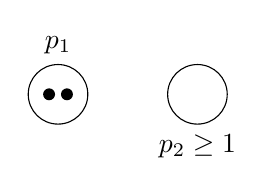
\begin{tikzpicture}
  \node[place,label=above:$p_1$,tokens=2]        (p1) {};
  \node[place,label=below:$p_2\ge1$,right=of p1] (p2) {};
\end{tikzpicture}
\end{codeexample}

    \begin{stylekey}{/tikz/every place}
        This style is evoked by the style |place|. To change the appearance of
        places, you can change this style.
        %
\begin{codeexample}[]
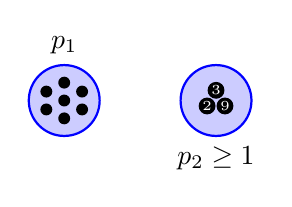
\begin{tikzpicture}
  [every place/.style={draw=blue,fill=blue!20,thick,minimum size=9mm}]
  \node[place,tokens=7,label=above:$p_1$]  (p1) {};
  \node[place,structured tokens={3,2,9},
        label=below:$p_2\ge1$,right=of p1] (p2) {};
\end{tikzpicture}
\end{codeexample}
    \end{stylekey}
\end{stylekey}


\subsection{Transitions}

Transitions are also nodes. They should be drawn using the following style:

\begin{stylekey}{/tikz/transition}
    This style indicates that a node is a transition. As for places, the text
    of a transition should be empty and the |label| option should be used for
    adding labels.

    To connect a transition to places, you can use the |edge| command as in the
    following example:
    %
\begin{codeexample}[]
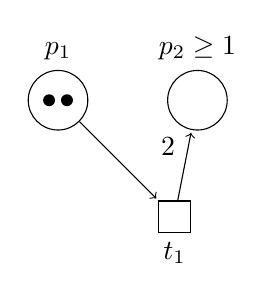
\begin{tikzpicture}
  \node[place,tokens=2,label=above:$p_1$]        (p1) {};
  \node[place,label=above:$p_2\ge1$,right=of p1] (p2) {};

  \node[transition,below right=of p1,label=below:$t_1$] {}
    edge[pre]                 (p1)
    edge[post] node[auto] {2} (p2);
\end{tikzpicture}
\end{codeexample}

    \begin{stylekey}{/tikz/every transition}
        This style is evoked by the style |transition|.
    \end{stylekey}

    \begin{stylekey}{/tikz/pre}
        This style can be used with paths leading \emph{from} a transition
        \emph{to} a place to indicate that the place is in the pre-set of the
        transition. By default, this style is |<-,shorten <=1pt|, but feel free
        to redefine it.
    \end{stylekey}

    \begin{stylekey}{/tikz/post}
        This style is also used with paths leading \emph{from} a transition
        \emph{to} a place, but this time the place is in the post-set of the
        transition. Again, feel free to redefine it.
    \end{stylekey}

    \begin{stylekey}{/tikz/pre and post}
        This style is to be used to indicate that a place is both in the pre-
        and post-set of a transition.
    \end{stylekey}
\end{stylekey}


\subsection{Tokens}
\label{section-tokens}

Interestingly, the most complicated aspect of drawing Petri nets in \tikzname\
turns out to be the placement of tokens.

Let us start with a single token. They are also nodes and there is a simple
style for typesetting them.

\begin{stylekey}{/tikz/token}
    This style indicates that a node is a token. By default, this causes the
    node to be a small black circle. Unlike places and transitions, it
    \emph{does} make sense to provide text for the token node. Such text will
    be typeset in a tiny font and in white on black (naturally, you can easily
    change this by setting the style |every token|).
    %
\begin{codeexample}[]
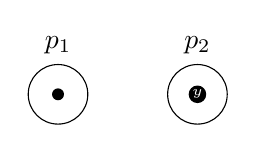
\begin{tikzpicture}
  \node[place,label=above:$p_1$]             (p1) {};
  \node[token] at (p1) {};

  \node[place,label=above:$p_2$,right=of p1] (p2) {};
  \node[token] at (p2) {$y$};
\end{tikzpicture}
\end{codeexample}
    %
    \begin{stylekey}{/tikz/every token}
        Change this style to change the appearance of tokens.
    \end{stylekey}
\end{stylekey}

In the above example, it is bothersome that we need an extra command for the
token node. Worse, when we have \emph{two} tokens on a node, it is difficult to
place both nodes inside the node without overlap.

The Petri net library offers a solution to this problem: The
|children are tokens| style.

\begin{stylekey}{/tikz/children are tokens}
    The idea behind this style is to use trees mechanism for placing tokens.
    Every token lying on a place is treated as a child of the node. Normally
    this would have the effect that the tokens are placed below the place and
    they would be connected to the place by an edge. The |children are tokens|
    style, however, redefines the growth function of trees such that it places
    the children next to each other inside (or, rather, on top) of the place
    node. Additionally, the edge from the parent node is not drawn.
    %
\begin{codeexample}[]
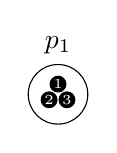
\begin{tikzpicture}
  \node[place,label=above:$p_1$] {}
  [children are tokens]
  child {node [token] {1}}
  child {node [token] {2}}
  child {node [token] {3}};
\end{tikzpicture}
\end{codeexample}

    In detail, what happens is the following: Tree growth functions tell
    \tikzname\ where it should place the children of nodes. These functions get
    passed the number of children that a node has an the number of the child
    that should be placed. The special tree growth function for tokens has a
    special mapping for each possible number of children up to nine children.
    This mapping decides for each child where it should be placed on top of the
    place. For example, a single child is placed directly on top of the place.
    Two children are placed next to each other, separated by the
    |token distance|. Three children are placed in a triangle whose side
    lengths are |token distance|; and so on up to nine tokens. If you wish to
    place more than nice tokens on a place, you will have to write your own
    placement code.
    %
\begin{codeexample}[]
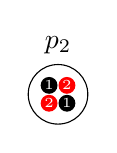
\begin{tikzpicture}
  \node[place,label=above:$p_2$] {}
  [children are tokens]
  child {node [token] {1}}
  child {node [token,fill=red] {2}}
  child {node [token,fill=red] {2}}
  child {node [token] {1}};
\end{tikzpicture}
\end{codeexample}

    \begin{key}{/tikz/token distance=\meta{distance}}
        This specifies the distance between the centers of the tokens in the
        arrangements of the option |children are tokens|.
        %
\begin{codeexample}[]
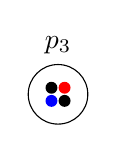
\begin{tikzpicture}
  \node[place,label=above:$p_3$] {}
  [children are tokens,token distance=1.1ex]
  child {node [token] {}}
  child {node [token,red] {}}
  child {node [token,blue] {}}
  child {node [token] {}};
\end{tikzpicture}
\end{codeexample}
    \end{key}
\end{stylekey}

The |children are tokens| option gives you a lot of flexibility, but it is a
bit cumbersome to use. For this reason there are some options that help in
standard situations. They all use |children are tokens| internally, so any
change to, say, the |every token| style will affect how these options depict
tokens.

\begin{key}{/tikz/tokens=\meta{number}}
    This option is given to a |place| node, not to a |token| node. The effect
    of this option is to add \meta{number} many child nodes to the place, each
    having the style |token|. Thus, the following two pieces of codes have the
    same effect:
    %
\begin{codeexample}[]
\tikz
  \node[place] {}
  [children are tokens]
  child {node [token] {}}
  child {node [token] {}}
  child {node [token] {}};
\tikz
  \node[place,tokens=3] {};
\end{codeexample}
    %
    It is legal to say |tokens=0|, no tokens are drawn in this case. This
    option does not handle ten or more tokens correctly. If you need this many
    tokens, you will have to program your own code.
    %
\begin{codeexample}[]
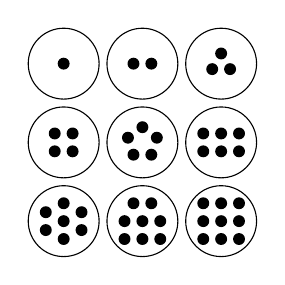
\begin{tikzpicture}[every place/.style={minimum size=9mm}]

  \foreach \x/\y/\tokennumber in {0/2/1,1/2/2,2/2/3,
                                  0/1/4,1/1/5,2/1/6,
                                  0/0/7,1/0/8,2/0/9}
    \node [place,tokens=\tokennumber] at (\x,\y) {};
\end{tikzpicture}
\end{codeexample}
    %
\end{key}

\begin{key}{/tikz/colored tokens=\meta{color list}}
    This option, which must also be given when a place node is being created,
    gets a list of colors as parameter. It will then add as many tokens to the
    place as there are colors in this list, each filled correspondingly.
    %
\begin{codeexample}[]
\tikz  \node[place,colored tokens={black,black,red,blue}] {};
\end{codeexample}
    %
\end{key}

\begin{key}{/tikz/structured tokens=\meta{token texts}}
    This option, which must again be passed to a place, gets a list of texts
    for tokens. For each text, a new token will be added to the place.
    %
\begin{codeexample}[]
\tikz  \node[place,structured tokens={$x$,$y$,$z$}] {};
\end{codeexample}
    %
\begin{codeexample}[]
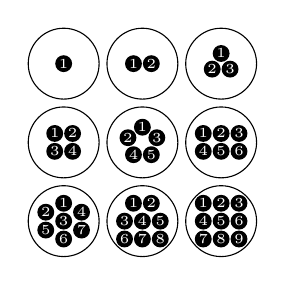
\begin{tikzpicture}[every place/.style={minimum size=9mm}]

  \foreach \x/\y/\tokennumber in {0/2/1,1/2/2,2/2/3,
                                  0/1/4,1/1/5,2/1/6,
                                  0/0/7,1/0/8,2/0/9}
    \node [place,structured tokens={1,...,\tokennumber}] at (\x,\y) {};
\end{tikzpicture}
\end{codeexample}
    %
    If you use lots of structured tokens, consider redefining the |every token|
    style so that the tokens are larger.
\end{key}


\subsection{Examples}

\begin{codeexample}[]
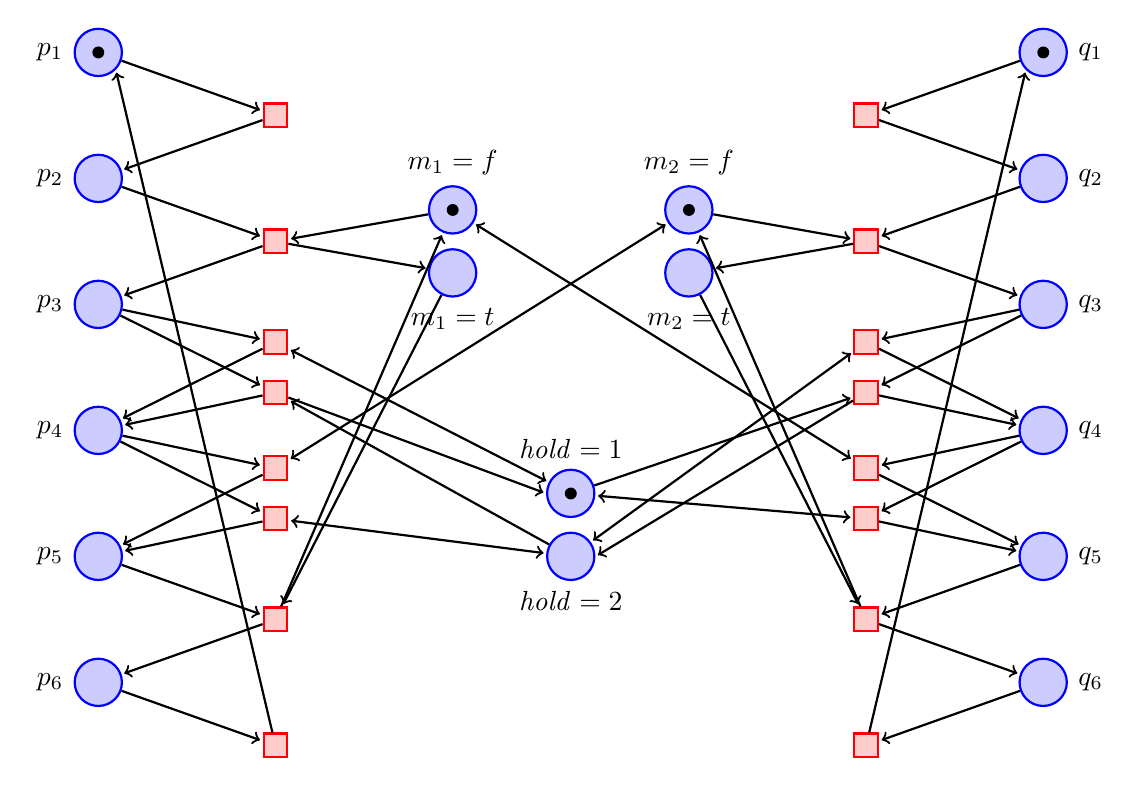
\begin{tikzpicture}[yscale=-1.6,xscale=1.5,thick,
  every transition/.style={draw=red,fill=red!20,minimum size=3mm},
  every place/.style={draw=blue,fill=blue!20,minimum size=6mm}]

  \foreach \i in {1,...,6} {
    \node[place,label=left:$p_\i$] (p\i) at (0,\i) {};
    \node[place,label=right:$q_\i$] (q\i) at (8,\i) {};
  }
  \foreach \name/\var/\vala/\valb/\height/\x in
      {m1/m_1/f/t/2.25/3,m2/m_2/f/t/2.25/5,h/\mathit{hold}/1/2/4.5/4} {
    \node[place,label=above:{$\var = \vala$}] (\name\vala) at (\x,\height) {};
    \node[place,yshift=-8mm,label=below:{$\var = \valb$}] (\name\valb) at (\x,\height) {};
  }
  \node[token] at (p1) {};   \node[token] at (q1) {};
  \node[token] at (m1f) {};  \node[token] at (m2f) {};
  \node[token] at (h1) {};

  \node[transition] at (1.5,1.5) {}  edge [pre] (p1)  edge [post] (p2);
  \node[transition] at (1.5,2.5) {}  edge [pre] (p2)  edge[pre]   (m1f)
                                     edge [post](p3)  edge[post]  (m1t);
  \node[transition] at (1.5,3.3) {}  edge [pre] (p3)  edge [post] (p4)
                                     edge [pre and post] (h1);
  \node[transition] at (1.5,3.7) {}  edge [pre] (p3)  edge [pre] (h2)
                                     edge [post] (p4) edge [post] (h1.west);
  \node[transition] at (1.5,4.3) {}  edge [pre] (p4)  edge [post] (p5)
                                     edge [pre and post] (m2f);
  \node[transition] at (1.5,4.7) {}  edge [pre] (p4)  edge [post] (p5)
                                     edge [pre and post] (h2);
  \node[transition] at (1.5,5.5) {}  edge [pre] (p5)  edge [pre] (m1t)
                                     edge [post] (p6) edge [post] (m1f);
  \node[transition] at (1.5,6.5) {}  edge [pre] (p6)  edge [post] (p1.south east);
  \node[transition] at (6.5,1.5) {}  edge [pre] (q1)  edge [post] (q2);
  \node[transition] at (6.5,2.5) {}  edge [pre] (q2)  edge [pre] (m2f)
                                     edge [post] (q3) edge [post] (m2t);
  \node[transition] at (6.5,3.3) {}  edge [pre] (q3)  edge [post] (q4)
                                     edge [pre and post] (h2);
  \node[transition] at (6.5,3.7) {}  edge [pre] (q3)  edge [pre] (h1)
                                     edge [post] (q4) edge [post] (h2.east);
  \node[transition] at (6.5,4.3) {}  edge [pre] (q4)  edge [post] (q5)
                                     edge [pre and post] (m1f);
  \node[transition] at (6.5,4.7) {}  edge [pre] (q4)  edge [post] (q5)
                                     edge [pre and post] (h1);
  \node[transition] at (6.5,5.5) {}  edge [pre] (q5)  edge [pre] (m2t)
                                     edge [post] (q6) edge [post] (m2f);
  \node[transition] at (6.5,6.5) {}  edge [pre] (q6)  edge [post] (q1.south west);
\end{tikzpicture}
\end{codeexample}

Here is the same net once more, but with these styles changes:
%
\begin{codeexample}[code only]
\begin{tikzpicture}[yscale=-1.1,thin,>=stealth,
  every transition/.style={fill,minimum width=1mm,minimum height=3.5mm},
  every place/.style={draw,thick,minimum size=6mm}]
\end{codeexample}

\begin{tikzpicture}[yscale=-1.1,thin,>=stealth,
  every transition/.style={fill,minimum width=1mm,minimum height=3.5mm},
  every place/.style={draw,thick,minimum size=6mm}]

  \foreach \i in {1,...,6} {
    \node[place,label=left:$p_\i$] (p\i) at (0,\i) {};
    \node[place,label=right:$q_\i$] (q\i) at (8,\i) {};
  }
  \foreach \name/\var/\vala/\valb/\height/\x in
      {m1/m_1/f/t/2.25/3,m2/m_2/f/t/2.25/5,h/\mathit{hold}/1/2/4.5/4} {
    \node[place,label=above:{$\var = \vala$}] (\name\vala) at (\x,\height) {};
    \node[place,yshift=-8mm,label=below:{$\var = \valb$}] (\name\valb) at (\x,\height) {};
  }
  \node[token] at (p1) {};   \node[token] at (q1) {};
  \node[token] at (m1f) {};  \node[token] at (m2f) {};
  \node[token] at (h1) {};

  \node[transition] at (1.5,1.5) {}  edge [pre]  (p1) edge [post] (p2);
  \node[transition] at (1.5,2.5) {}  edge [pre]  (p2) edge [pre]  (m1f)
                                     edge [post] (p3) edge [post] (m1t);
  \node[transition] at (1.5,3.3) {}  edge [pre]  (p3) edge [post] (p4)
                                     edge [pre and post]          (h1);
  \node[transition] at (1.5,3.7) {}  edge [pre]  (p3) edge [pre]  (h2)
                                     edge [post] (p4) edge [post] (h1.west);
  \node[transition] at (1.5,4.3) {}  edge [pre]  (p4) edge [post] (p5)
                                     edge [pre and post]          (m2f);
  \node[transition] at (1.5,4.7) {}  edge [pre]  (p4) edge [post] (p5)
                                     edge [pre and post]          (h2);
  \node[transition] at (1.5,5.5) {}  edge [pre]  (p5) edge [pre]  (m1t)
                                     edge [post] (p6) edge [post] (m1f);
  \node[transition] at (1.5,6.5) {}  edge [pre]  (p6) edge [post] (p1.south east);
  \node[transition] at (6.5,1.5) {}  edge [pre]  (q1) edge [post] (q2);
  \node[transition] at (6.5,2.5) {}  edge [pre]  (q2) edge [pre]  (m2f)
                                     edge [post] (q3) edge [post] (m2t);
  \node[transition] at (6.5,3.3) {}  edge [pre]  (q3) edge [post] (q4)
                                     edge [pre and post]          (h2);
  \node[transition] at (6.5,3.7) {}  edge [pre]  (q3) edge [pre]  (h1)
                                     edge [post] (q4) edge [post] (h2.east);
  \node[transition] at (6.5,4.3) {}  edge [pre]  (q4) edge [post] (q5)
                                     edge [pre and post]          (m1f);
  \node[transition] at (6.5,4.7) {}  edge [pre]  (q4) edge [post] (q5)
                                     edge [pre and post]          (h1);
  \node[transition] at (6.5,5.5) {}  edge [pre]  (q5) edge [pre]  (m2t)
                                     edge [post] (q6) edge [post] (m2f);
  \node[transition] at (6.5,6.5) {}  edge [pre]  (q6) edge [post] (q1.south west);
\end{tikzpicture}


%%% Local Variables:
%%% mode: latex
%%% TeX-master: "pgfmanual-pdftex-version"
%%% End:
